\documentclass[a4paper]{article}
    \usepackage[margin=0.25in]{geometry}
    \usepackage{multicol}
    \usepackage{graphicx}

    \begin{document}
    \begin{multicols}{2}
        \scriptsize
        \noindent\textbf{Algorithm}: precise, unambiguous, step by step procedure for carrying out some calculation or more generally for solving some problem\\
        \textbf{Algorithmics}: study of algorithms (design \& analysis)\\
        \textbf{Algorithm Properties}: Input, Output, Precision, Determinism, Finiteness, Correctness, Generality\\
        \textbf{Algorithm Creation Process}: understand, design, analyse (possibly back to design), implement\\
        \textbf{Analysis}: correctness, termination, simplicity, generality, time, space\\
        \textbf{Logarithms}: $b^e = x$ iff $\log_b x = e$; $\log xy = \log x + \log y$, $x, y > 0$; $\log \frac{x}{y} = \log x - \log y$, $x, y > 0$; $\log_b x^y = y \log_b x$; $\log_a x = \frac{\log_b x}{\log_b a}, a > 0, a \neq 1$; $\log_b x > \log_b y, b > 1, x > y > 0$\\
        \textbf{Series}: $\sum\nolimits_{i=1}^n i = \frac{n(n+1)}{2} = \Theta (n^2)$; $\sum\nolimits_{i=1}^n i^2 = \frac{n(n+1)(2n+1)}{6} = \Theta (n^3)$; $\sum\nolimits_{i=1}^n i^3 = {(\sum\nolimits_{i=1}^n i)}^2 = \Theta (n^4)$; $\sum\nolimits_{i=1}^n i^k \approx \frac{n^{k+1}}{k+1} = \Theta (n^{k+1})$; $\sum\nolimits_{i=0}^n a^i = \frac{a^{n+1}-1}{a-1} = \Theta (a^n)$; $\sum\nolimits_{i=1}^n i2^i = (n-1)2^{n+1}+2 = \Theta (n2^n)$; $\sum\nolimits_{i=1}^n \frac{1}{i} \approx \ln n + 0.57 = \Theta (\lg n)$; $\sum\nolimits_{i=1}^n \lg i = \Theta (n \lg n)$; $\sum\nolimits_{i=1}^n i \lg i = \Theta (n^2 \lg n)$\\
        \textbf{Theorem}: mathematical statement that has been proved true\\
        \textbf{Lemma}: `small' theorem, usually used in proof of a more important mathematical statement\\
        \textbf{Corollary}: mathematical statement which easily follows from a theorem\\
        \textbf{Proof}: logical argument that a mathematical statement is true\\
        \textbf{Proof by Construction}: mathematical statement about the existence of an object can be proved by constructing the object\\
        \textbf{Proof by Contradiction}: assume that a mathematical statement is false and show that the assumption leads to a contradiction\\
        \textbf{Polynomial Degree}: highest power\\
        \textbf{Intervals}: closed ($[a,b] = x | a \leq x \leq b$), open ($(a,b) = x | a < x < b$), half-open (either side)\\
        \textbf{Subsequence}: consists of only certain terms in the same order as the full sequence\\
        \textbf{Substring}: assume string index start from 1, then for $t[i,j]$ if $i < j$ then substring is from $i$ to $j$ inclusive, if $i = j$ then substring is only $i$, else then empty string\\
        \textbf{Boolean Expression}: containing boolean variables, operators, parentheses\\
        \textbf{Normal Forms}: conjunctive (clause linked with $\wedge$, inside has $\vee$), disjunctive (opposite)\\
        \textbf{Upper Bound}: $u$ such that $x \leq u$ for all $x \in X$, $X$: all reals\\
        \textbf{Lower Bound}: $l$ such that $x \geq l$ for all $x \in X$\\
        \textbf{Supremum}: least upper bound\\
        \textbf{Infimum}: greatest lower bound\\
        \textbf{Graph}: consists of set of vertices and edges, edge is unordered (unless directed) pair of vertices, simple if without loops or multiple edges\\
        \textbf{Degree}: number of edges incident on the vertex\\
        \textbf{Path}: alternating sequence of vertices and edges, starting and ending with vertices, simple has no repeated vertices\\
        \textbf{Diameter}: maximum distance between any two vertices\\
        \textbf{Cycle}: path starting and ending at the same vertex with actual length, simple if without repeated vertices\\
        \textbf{Hamiltonian Cycle}: cycle that contains each vertex exactly once\\
        \textbf{Euler Cycle}: cycle with no repeated edges that contains all edges and vertices, exists iff connected and degree of every vertex is even\\
        \textbf{Complement}: of simple graph, denoted as $\bar{G}$, same vertices, edge in $\bar{G}$ iff not in $G$\\
        \textbf{Tree}: connected and acyclic; connected and has $n - 1$ edges, acyclic and has $n - 1$ edges, level of vertex is simple path length from root, height is max length\\
        \textbf{Homogeneous Recurrence}: characteristic equation ($a_0t_n + a_1t_{n-1} + \cdots + a_k t_{n-k} = 0$) linear, homogeneous (combination of $t_i = 0$), constant coefficients, guess $t_n = x^n$, unknown x, so $a_0x^n + a_1x^{n-1} + \cdots + a_k x^{n-k} = 0$, factor out $x^{n-k}$, so $p(x) = a_0x^k + a_1x^{k-1} + \cdots + a^k x^0 = 0$, so the general solution is $\sum\nolimits_{i=1}^k c_i r_i^n$, where $r$ is the roots of the equation (if distinct)\\
        \textbf{HR Example}: $T(n) = 2T(n-1), T(1) = 1, T(n) - 2T(n-1) = 0, T(n) = x^n, T(n-1) = x^{n-1}$, solve $x^n-2x^{n-1} = 0, x = 2, T(n) = c_1 2^n, T(1) = 1 = c_1 2^1, c_1 = 0.5$\\
        \textbf{HR with Non Distinct Roots}: for each non distinct root include it but multiply with n each time ($c_1r^n+c_2nr^n+c_3n^2r^n+\cdots$)\\
        \underline{\textbf{Asymptotic Upper Bound}}: $f(n = O(g(n)))$ if there exist $C_1 > 0$ and $N_1$ such that $f(n) \leq C_1g(n), n \geq N_1$\\
        \textbf{Asymptotic Lower Bound}: $f(n) = \Omega (g(n))$ if there exist $C_2 > 0$ and $N_2$ such that $f(n) \geq C_2g(n), n \geq N_2$\\
        \textbf{Master Theorem}: $T(n) = aT(n/b)+f(n), f(n) = \Theta (n^k)$, $T(n) = \Theta (n^k)$ if $a < b^k$, $T(n) = \Theta (n^k \log n)$ if $a = b^k$, $T(n) = \Theta (n^{\log_b a})$ if $a > b^k$\\
        \textbf{Smoothness}: if the function is non decreasing from N inclusive to infinity, and for every integer $b \geq 2, f(bn) = O(f(n))$\\
        \textbf{Formal Smoothness}: for any integer $b \geq 2, C > 0, N > 0, f(bn) \leq Cf(n), f(n) \leq f(n+1)$, for all $n \geq N$\\
        \underline{\textbf{Binary Tree Traversal}}: preorder (root, left, right), inorder (left, root, right), postorder (left, right, root)\\
        \textbf{Binary Search Tree}: to insert search through and put in spot where it would be, to delete node with 0 or 1 child simply delete like linked list, else find minimum in right subtree, swap with target, and delete\\
        \textbf{Heap}: if array start from 1 then left child is $2i$, right child is $2i+1$, to siftdown maxheap get larger child, if child is larger than current move child up, look at next child, to delete swap last in array with target, siftdown swapped, to insert do so at end, then siftup (if current is greater than parent move parent down, look at next parent), to heapify do siftdown from $i = n/2 \to 1$\\
        \textbf{Heap Complexities}: lg n for delete, insert (O only), \& siftdown (tree height), n for heapify\\
        \textbf{Indirect Heap}: key, into (key index into heap index), outof (heap index into key index), whenever setting outof[x] = y also set into[y] = x, for increase/decreaseKey just siftup the modified node\\
        \textbf{Heapsort}: heapify (maxheap), largest element is in the first, swap with last in the heap, decrease the heap length, siftdown on root, repeat until heap has only 1 element (which would be minimum)\\
        \textbf{Disjoint Sets}: stored as array of parents, parent[i] is the parent of element i, makeset (constructs new set with one element from parameter, set parent to itself), findset (returns the marked member of the set containing parameter, keep going through parent, while doing so check the node parent, if not root make it root and continue to next parent), union (replace sets containing the parameters with the union, find the sets of both and make one of the sets the parent of the other, use the deepest tree as the parent)\\
        \underline{\textbf{Interpolation Search}}: estimates where the search key is in the array, assumes values in array increase linearly with index, worst case n but with random keys average case is lg lg n\\
        \textbf{Hashing}: average $1 + \frac{n}{2m}$\\
        \underline{\textbf{Topological Sort}}: DFS, but for every dead end (all incident vertices visited already) add to head of list\\
        \textbf{Depth First Search}: set visit to false for all, then for each unvisited node run recursive (in case of disconnected graph), in recursive set visit to true for the vertex and recurse on all adjacent (if not visited), complexity is $\Theta (|V| + |E|)$ for adjacency list, with adjacency matrix is $\Theta (|V|^2)$ (to get adjacent vertices need to go through whole row/column)\\
        \textbf{DFS Applications}: find spanning trees, connected components, cut vertices/articulation points, exploring graphs, topological sort, backtracking\\
        \textbf{Breadth First Search}: same as DFS for starting, but instead of recursive set current visit to true, add current to queue, for all in queue dequeue, then for each adjacent to dequeued if was not visited then visit and enqueue, complexity same as DFS\\
        \textbf{BFS Applications}: find spanning trees, connected components, shortest path, exploring graphs, web crawling, social networking, garbage collection, puzzles, games\\
        \underline{\textbf{Mergesort}}: to merge just compare first element of both lists, get smallest one and put into new list, if one emptied then just grab all from the other, main method simply splits the list into 2, recurse on both, then merge, is stable\\
        \textbf{Bubblesort}: start from end, keep swapping if out of order, after each pass will get smallest at the start, keep going while ignoring the ones at the start (already sorted), $n^2$, stable\\
        \textbf{Insertion sort}: start with sorted list of 1 element (the first), then insert a[2] into the sorted list (only a[1]), then insert a[3] into the sorted list of a[1], a[2], and so on, $n^2$, stable\\
        \textbf{Quicksort}: partition (values before partition is less than, values after partition is greater than or equal to, goes through the whole portion), then recurse on the halves before and after the partition, worst $n^2$, but average with random partition n log n, not stable\\
        \textbf{Counting Sort}: init count array, count how many times index appears in actual array, convert count array to cumulative, get cumulative count per element and use it as index in new array, subtract the count (for duplicates), copy new array to original, complexity n + m, range from 0 to m, stable\\
        \textbf{Radix Sort}: use counting sort on each digit, complexity is kn, k is max number of digits, stable\\
        \textbf{Random Select}: worst case $n^2$, average $n$\\
        \underline{\textbf{Greedy Algorithms}}: on each step make choice that is feasible (satisfy constraint), locally optimal (best among all feasible choices), irrevocable (no backtracking)\\
        \textbf{Kruskal's Algorithm}: greedy by edges, start with all vertices but no edges, sort edgelist, if adding smallest edge does not create cycle (the vertices being connected are not in the same disjoint set) then add (union the sets the vertices are in), otherwise skip it, stop when n-1 edges added, $\Theta |E| \log n$ (sort is $|E| \log |E|$, $\log |E| = \Theta (\log n)$, each findset/union takes $O(\log n$))\\
        \textbf{Prim's Algorithm}: start with 1 vertex and no edges, find minimum weight edge among all edges leaving the tree (can keep track of the distance to the tree per vertex and the nearest tree vertex), add it to the tree (after adding need to update vertices around the new one if the distance is now shorter, also update parent), stop when all vertices added, $O(|E| \log n)$ (if using adjacency list and heap, n for heapify, log n for every poll, also decreaseKey per edge possibly, which is where it comes from)\\
        \textbf{Dijkstra's Algorithm}: init all priorities of vertices to infinity, put in priority queue, decreaseKey on the start with distance 0, dequeue vertex from queue, add it to tree, for every vertex adjacent to new one update distance where necessary, decreaseKey and set parent, do so until we have all vertices or we found the vertex we want\\
        \underline{\textbf{Principle of Optimality}}: required for dynamic programming, if we have a set of optimal solutions to a group of sub-problems, and we have an optimal method of combining solutions, then we have an optimal solution to a problem made up from the sub problems\\
        \textbf{Warshall's Algorithm}: compute transitive closure of a directed graph (matrix where t[i][j] = 1 iff there is a directed nontrivial path from vertex i to vertex j), create series of matrices M\textsubscript{k} from 1 to n, in M\textsubscript{k}, m[i][j] = 1 iff there is a directed path from i to j such that no vertex on the path has label greater than k, so to get next matrix m[i][j] = 1 if it was 1 before or if both m[i][k] and m[k][j] is 1 (meaning there is a path if we allow going through k), complexity is $\Theta (n^3)$\\
        \textbf{Floyd's Algorithm}: compute matrix where m[i][j] contains the shortest distance from vertex i to j (directed graph), similar to Warshall's with 3 loops, but when updating compare a[i][j] (current without k) and a[i][k] + a[k][j] (include k), store shorter one, when initializing go through edges and note down the distances, if no edge then set to infinity, same complexity as Warshall's\\
        \textbf{Binomial Coefficients}: $C(n, k) = C(n-1, k-1) + C(n-1, k), n > k > 0, C(n,0) = C(n,n) = 1$\\
        \underline{\textbf{NP}}: class of decision problems that have polynomial time verifiers, decided by nondeterministic polynomial time Turing machine\\
        \textbf{Clique}: in undirected graph is a subgraph such that every 2 vertices in the clique are connected by an edge, k-clique is a clique with k vertices, finding k-clique is NP (to verify check if the set of vertices is a set of k vertices in the graph, then check if every 2 vertices are connected by an edge, complexity would be $n^2$, since $C(n, 2) = \frac{n(n-1)}{2}$)\\
        \textbf{Independent Set}: set of vertices such that no two of them are adjacent, NP-complete\\
        \textbf{Subset-Sum}: find a subset where the sum is a given number, is also NP\\
        \textbf{NP-complete}: if polynomial time algorithm exists for any of these problems, all problems in NP would have polynomial time algorithm (if B is NP-complete and B is in P then P = NP), B is NP-complete if B is in NP and $A \leq_p B$ for all A in NP, if B is NP-complete and $B \leq_p C$ and C is in NP then C is NP-complete\\
        \textbf{Polynomial Time Reducible}: $A \leq_p B$ if there is a polynomial time reduction (mapping from instances of A to instanes of B such that every yes instance of A is reduced to a yes instance of B, and the same for no instances) from A to B, if $A \leq_p B \wedge B \in P \to A \in P$\\
        \textbf{3SAT}: SAT with 3 clause conjunctive normal form, to prove NP-complete prove 3SAT is NP (just check every clause) and reduce SAT to 3SAT (below), also need to prove that reduction is polynomial (for each clause with $k$ literals, $k \geq 4$, $k$ clauses, since $k \leq 2n$, no more than $2mn$ clauses, $m$ is the number of clauses, $n$ is the number of literals)\\
        \textit{1 literal}: replace $(x)$ with $(x, y_1, y_2), (x, \bar{y_1}, y_2), (x, y_1, \bar{y_2}), (x, \bar{y_1}, \bar{y_2})$, for any assignment to $y_1$ and $y_2$ there will always be on unsatisfied clause, so $x$ has to be true for the clause to be satisfied\\
        \textit{2 literals}: replace $(x_1, x_2) $with $(x_1, x_2, y), (x_1, x_2, \bar{y})$\\
        \textit{3+ literals}: replace $(x_1, \ldots, x_k)$ with $(x_1, x_2, \bar{y_1}), (y_1, x_3, \bar{y_2}), (y_2, x_4, \bar{y_3}), \ldots, \\(y_{k-3}, x_{k-1}, x_k)$\\
        \underline{\textbf{Proving NP-Completeness}}: Restriction (if special case of problem is NP-complete, so need to prove that the problem is in NP, then reduce an arbitrary instance of the special case to the target problem), Local Replacement (each component of the problem is replaced locally by a collection of components, and there is no added interaction between components, e.g. SAT to 3SAT, Hamiltonian circuit to TSP), Component Design (more complicated types of reduction, where there is interaction between construction components)\\
        \textbf{Local Replacement Example}: prove TSP is NP-complete using Hamiltonian circuit (known NP-complete), take an instance of Hamiltonian circuit (a graph G), then construct a complete weighted graph G', each vertex in G has a corresponding vertex in G', if an edge is in G then the corresponding edge in G' has weight 1, else then it has weight 2, then G' has a route of length $|V|$ (meaning that the route covers all vertices) iff G has Hamiltonian circuit\\
        \textbf{Approximation Algorithms}: runs in polynomial time and finds solution that is close to optimal, performance ratio is the ratio of the approximation solution over the optimal solution (opposite if maximisation problem), constant factor has performance ratio bounded by constant\\
        \textbf{Vertex Cover}: given graph, is there a subset of vertices of size k that every edge has at least one end vertex in cover\\
        \textbf{Vertex Cover Approximation}: factor 2, while there are still edges left select an edge, add its ends to the set of vertices, delete the new vertices and all incident edges to both\\
        \textbf{Proof of no Constant Factor Approximation for TSP if $P \neq NP$}: assume it exists with factor c, then we can use that to solve Hamiltonian circuit in polynomial time (map instance of Hamiltonian (G) to TSP (G') similar to local replacement, but instead of 2 if nonexistent edge use cn+1, if there is Hamiltonian circuit in G then optimal solution to TSP is the circuit with length n, since approximation will find a solution with length $\leq cn$, it means it can't use any edge not in G if Hamiltonian circuit exists, if there is no Hamiltonian circuit then it is forced to use a nonexistent edge from G, so the length will be $\geq cn+1$, so we can solve Hamiltonian circuit using the approximation algorithm by checking the length, if it is $\leq cn$ then there is a Hamiltonian circuit, else there is none), implying P = NP\\
        \textbf{Heuristics}: algorithm based on exploration \& trial \& error, typically do not have performance guarantees, e.g.\ greedy for TSP\\
        \textbf{Restriction}: to special cases which do have polynomial time algorithm or a constant factor approximation, e.g.\ restrict TSP to Euclidean (direct road is always shorter than going through another vertex on the way), find minimum spanning tree, start DFS from a vertex, record traversed vertices in list (including when backtracking), go through the list and remove duplicates after the first one (taking shortcut), remaining vertex order is the cycle, at most 2x as long as minimum\\
        \textbf{Parameterization}: focus on instances that are not necessarily small but have a small parameter, ideally with running time of $O(f(k)n^c)$, where c is a small constant, $f(k)$ can even be exponential, if possible then Fixed Parameter Tractable, e.g.\ vertex cover of size k, can always just get vertex subsets of size k, remove all connected edges and see if there are any edges left, only $C(n, k) \in O(n^k)$, checking whether there are any edges left after removing the subset takes $O({(n-k)}^2)$, so total time is $O(n^{k+2})$\\
        \textbf{Vertex Cover FPT Example 2}: if k = 0 or no more edges return edges.isEmpty, else pick an edge (u, v), create G1 with u and incident edges removed, do the same with v for G2, return rec (G1, k-1) or rec (G2, k-1), complexity is $O(2^k (|V|+|E|))$\\
        \underline{\textbf{Text Searching}}: with basic worst case for n string and m pattern is $\Theta(m(n-m+1))$ if no pattern match, with random test and patterns takes $\Theta(n-m)$, ineffective for longer patterns and when particularly when text contains repeated elements $\Theta(n^2), m=n/2$\\
        \textbf{Rabin-Karp Algorithm}: compute hash/fingerprint table, then instead of checking every substring check fingerprint first (using mod, convert the binary string to number and mod with prime larger than the pattern), $\Theta(n+m)$ expected running time now, worst case same as basic\\
        \textbf{Knuth-Morris-Pratt Algorithm}: use shift table to skip characters already checked and known to not match, whole algorithm takes $O(m+n)$, shift table making takes $O(m)$\\
        \underline{\textbf{Coin-Weighing Problem}}:\\
        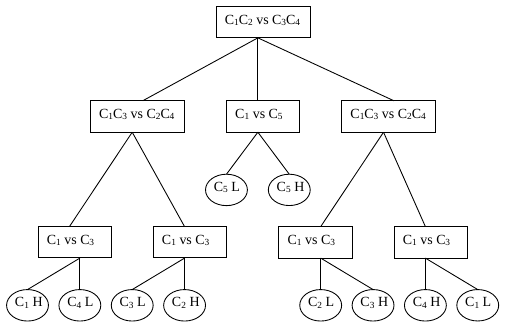
\includegraphics[width=\linewidth]{coinweigh.png}\\
    \end{multicols}
    \end{document}
